\section{Search Route Optimization and Heuristic Evaluation}

When human operators enter multiple search sectors, the transit sequence directly impacts total flight distance and mission duration. MANAR incorporates a deterministic nearest-neighbor route planner within the C++ control core. Fig.~\ref{fig:lawnmower_and_route} illustrates the spatial sweep geometry and waypoint routing graph.

\begin{figure}[t]
\centering
\resizebox{\columnwidth}{!}{%
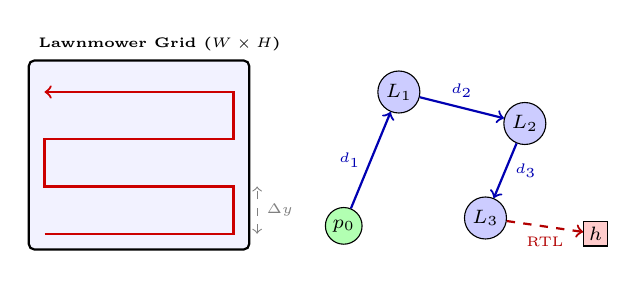
\begin{tikzpicture}[font=\sffamily\scriptsize]
    % Lawnmower grid on left
    \draw[thick, fill=blue!5, rounded corners=2pt] (0,0) rectangle (2.8,2.4);
    \node[anchor=south west, font=\tiny\bfseries] at (0,2.4) {Lawnmower Grid ($W \times H$)};
    \draw[->, thick, red!80!black] (0.2,0.2) -- (2.6,0.2) -- (2.6,0.8) -- (0.2,0.8) -- (0.2,1.4) -- (2.6,1.4) -- (2.6,2.0) -- (0.2,2.0);
    \draw[<->, dashed, gray] (2.9,0.2) -- (2.9,0.8) node[midway, right, font=\tiny] {$\Delta y$};

    % Route on right
    \begin{scope}[xshift=4.0cm, yshift=0.1cm]
        \node[draw, circle, fill=green!30, inner sep=1.5pt] (p0) at (0,0.2) {$p_0$};
        \node[draw, circle, fill=blue!20, inner sep=1.5pt] (L1) at (0.7,1.9) {$L_1$};
        \node[draw, circle, fill=blue!20, inner sep=1.5pt] (L2) at (2.3,1.5) {$L_2$};
        \node[draw, circle, fill=blue!20, inner sep=1.5pt] (L3) at (1.8,0.3) {$L_3$};
        \node[draw, rectangle, fill=red!20, inner sep=2pt] (home) at (3.2,0.1) {$h$};

        \draw[->, thick, blue!70!black] (p0) -- node[left, font=\tiny] {$d_1$} (L1);
        \draw[->, thick, blue!70!black] (L1) -- node[above, font=\tiny] {$d_2$} (L2);
        \draw[->, thick, blue!70!black] (L2) -- node[right, font=\tiny] {$d_3$} (L3);
        \draw[->, thick, dashed, red!70!black] (L3) -- node[below, font=\tiny] {RTL} (home);
    \end{scope}
\end{tikzpicture}%
}
\caption{Spatial geometry: Lawnmower sweep coverage pattern (left) and sequential greedy route progression with RTL return leg (right).}
\label{fig:lawnmower_and_route}
\end{figure}

\subsection{Problem Formulation \& Heuristic Selection}
Let an operator designate an unordered set of $n$ target search locations $L = \{L_1, L_2, \dots, L_n\}$, with $L_i = (\phi_i, \lambda_i)$. Let $p_0 = (\phi_{\mathrm{drone}}, \lambda_{\mathrm{drone}})$ denote initial position and $h = (\phi_{\mathrm{home}}, \lambda_{\mathrm{home}})$ denote home base coordinates. Finding the globally minimal tour through $n$ arbitrary points is an instance of the metric Traveling Salesperson Problem (TSP)~\cite{applegate2006traveling}, requiring $n!$ route evaluations under brute-force search.

For embedded mission initialization where candidate sectors are modest ($n \le 20$), MANAR selects the classical $O(n^2)$ greedy nearest-neighbor heuristic. Starting from $p_0$, the planner iteratively selects the closest unvisited location under Haversine distance:
\begin{equation}
p_{k+1} = \underset{x \in U_k}{\operatorname{argmin}} \; d(p_k, x), \quad k = 0, 1, \dots, n-1
\end{equation}
where $U_k$ is the unvisited set ($U_0 = L$, $U_{k+1} = U_k \setminus \{p_{k+1}\}$). The home base $h$ is appended solely as the final Return-to-Launch return leg $d(p_n, h)$:
\begin{equation}
d_{\mathrm{total}} = d(p_0, p_1) + \sum_{k=1}^{n-1} d(p_k, p_{k+1}) + d(p_n, h)
\end{equation}

\begin{table}[t]
\caption{Fixed-Seed Route Evaluation: Greedy vs.\ 2-Opt Refinement}
\label{tab:route_benchmark}
\centering
\scriptsize
\begin{tabular*}{\columnwidth}{@{\extracolsep{\fill}}rrrrr@{}}
\toprule
\textbf{$n$} & \textbf{Trials} & \textbf{Greedy} & \textbf{2-Opt} & \textbf{Relative Excess} \\
 & & \textbf{Mean (km)} & \textbf{Mean (km)} & \textbf{Mean $\pm$ SD (Max)} \\
\midrule
5 & 100 & 11.42 & 10.92 & $4.63\% \pm 5.30\%$ (22.31\%) \\
8 & 100 & 14.75 & 13.69 & $7.97\% \pm 7.41\%$ (29.46\%) \\
10 & 100 & 16.15 & 14.90 & $8.61\% \pm 8.12\%$ (31.21\%) \\
15 & 100 & 19.50 & 17.96 & $8.56\% \pm 7.13\%$ (26.40\%) \\
20 & 100 & 21.81 & 19.63 & $11.09\% \pm 7.63\%$ (32.80\%) \\
\bottomrule
\end{tabular*}
\end{table}

\subsection{Fixed-Seed Reference Evaluation}
The reproducibility script \texttt{reproducibility/route\_benchmark.py} evaluates 500 layouts using Python's fixed pseudorandom seed 20,260,815. For each $n \in \{5,8,10,15,20\}$, 100 target sets are sampled uniformly in a $5\text{ km}\times5\text{ km}$ square centered at $(25.2048^{\circ},55.2708^{\circ})$. Start and home coincide at the square center. Each nearest-neighbor tour is refined by repeated best-improvement 2-opt edge reversal until no improving reversal remains. The committed CSV contains the unrounded aggregate values.

The reported relative excess is
\begin{equation}
g_{\mathrm{2opt}} = 100\left(\frac{d_{\mathrm{greedy}}}{d_{\mathrm{2opt}}}-1\right)\%.
\end{equation}
This quantity is \emph{not} an optimality gap: 2-opt is a local heuristic and can itself remain above the global optimum. Exact TSP comparison for small $n$ is future work.

As summarized in Table~\ref{tab:route_benchmark}:
\begin{enumerate}
    \item \textbf{Route quality:} Mean excess over the 2-opt-refined reference rises from $4.63\%$ at $n=5$ to $11.09\%$ at $n=20$. The non-monotonic $n=10$ and $n=15$ means show that a fixed number of random layouts should not be overinterpreted as a smooth complexity law.
    \item \textbf{Tail behavior:} Worst observed excess ranges from $22.31\%$ to $32.80\%$, so nearest-neighbor ordering can be materially worse even when its average is moderate.
    \item \textbf{Runtime scope:} This reference script deliberately omits timing because Python runtime would not establish the C++ implementation's latency. A C++ benchmark must disclose compiler, optimization flags, processor, warm-up, repetitions, and raw samples before a microsecond claim is restored.
\end{enumerate}

\subsection{Tactical Operator Override Privilege}
In practical SAR missions, human domain intelligence (e.g., wind drift, survivor travel vectors, sun angle, or terrain barriers) frequently dictates a search sequence that differs from purely geometric proximity. Crucially, MANAR formalizes this via an explicit \textbf{Operator Override Privilege} toggle ($Y/N$). If the operator accepts optimization ($Y$), the greedy sequence executes; if the operator rejects optimization ($N$), the manual entry order ($p_k = L_k$) is strictly preserved. In both cases, submitting the plan locks the mission configuration (\texttt{searchplanlocked = true}), preventing in-flight race conditions or unexpected waypoint mutations.
